\documentclass{standalone}
\usepackage{tikz}
\usetikzlibrary{arrows.meta, positioning}

\begin{document}

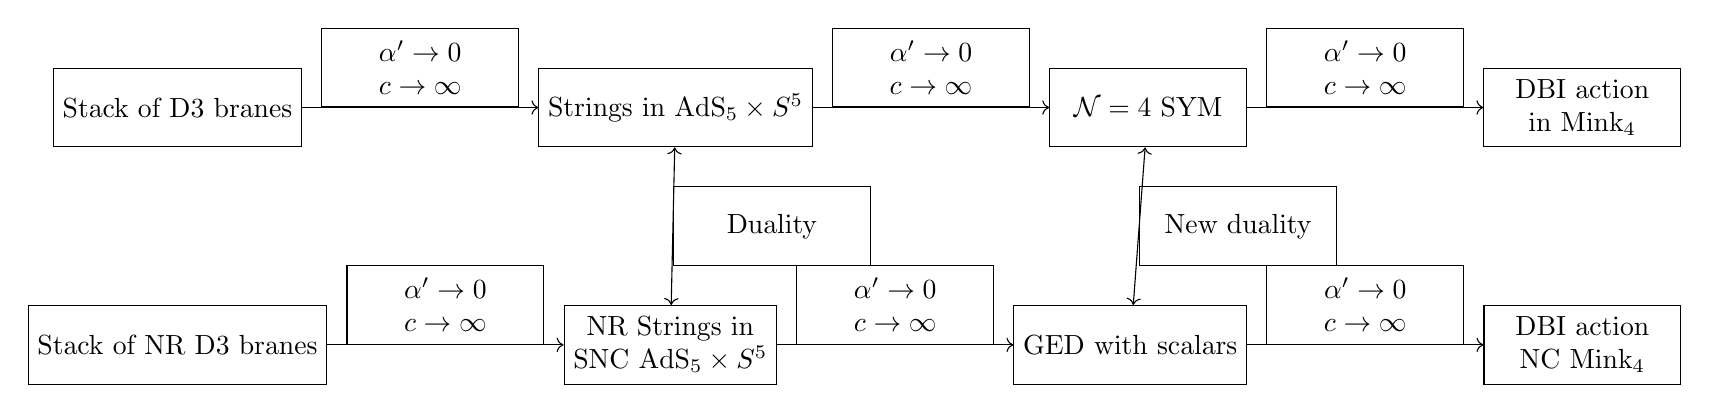
\begin{tikzpicture}[node distance=3cm, every node/.style={rectangle, draw, minimum height=1cm, minimum width=2.5cm, align=center}]

% Nodes
\node (A) {Stack of D3 branes};
\node (B) [right=of A] {Strings in AdS$_5 \times S^5$};
\node (C) [right=of B] {$\mathcal{N} = 4$ SYM};
\node (D) [right=of C] {DBI action \\ in Mink$_4$};

\node (E) [below=2cm of A] {Stack of NR D3 branes};
\node (F) [right=of E] {NR Strings in \\ SNC AdS$_5 \times S^5$};
\node (G) [right=of F] {GED with scalars};
\node (H) [right=of G] {DBI action \\ NC Mink$_4$};

% Arrows top row
\draw[->] (A) -- node[above] {$\alpha' \to 0$ \\ $c \to \infty$} (B);
\draw[->] (B) -- node[above] {$\alpha' \to 0$ \\ $c \to \infty$} (C);
\draw[->] (C) -- node[above] {$\alpha' \to 0$ \\ $c \to \infty$} (D);

% Arrows bottom row
\draw[->] (E) -- node[above] {$\alpha' \to 0$ \\ $c \to \infty$} (F);
\draw[->] (F) -- node[above] {$\alpha' \to 0$ \\ $c \to \infty$} (G);
\draw[->] (G) -- node[above] {$\alpha' \to 0$ \\ $c \to \infty$} (H);

% Duality arrows
\draw[<->] (B) -- node[right] {Duality} (F);
\draw[<->] (C) -- node[right] {New duality} (G);

\end{tikzpicture}

\end{document}